\documentclass[letterpaper]{jpconf}

\usepackage{graphicx}

\usepackage{hyperref}

\usepackage{cite}

\newcommand{\maestro}{{\sffamily Maestro}}
\newcommand{\castro}{{\sffamily Castro}}
\newcommand{\starkiller}{{\sffamily StarKiller}}
\newcommand{\starlord}{{\sffamily StarLord}}
\newcommand{\nyx}{{\sffamily Nyx}}
\newcommand{\amrex}{{\sffamily AMReX}}


\usepackage{color}
\setlength{\marginparwidth}{0.75in}
\newcommand{\MarginPar}[1]{\marginpar{\vskip-\baselineskip\raggedright\tiny\sffamily\hrule\smallskip{\color{red}#1}\par\smallskip\hrule}}



\begin{document}

\title{Meeting the Challenges of Modeling Astrophysical Thermonuclear Explosions:
\castro, \maestro, and the \amrex\ Astrophysics Suite}

\author{M. Zingale$^1$,
        A.~S. Almgren$^2$,
        M.~G. Barrios Sazo$^1$,
        V.~E. Beckner$^2$,
        J.~B. Bell$^2$,
        B. Friesen$^2$,
        A.~M. Jacobs$^3$,
        M.~P. Katz$^4$,
        C.~M. Malone$^5$,
        A.~J. Nonaka$^2$,
        D. Willcox$^1$, and
        W. Zhang$^2$}

\address{$^1$Department of Physics and Astronomy, Stony Brook
  University, Stony Brook, NY 11794-3800 USA}

\address{$^2$Center for Computational Sciences and Engineering,
  Lawrence Berkeley National Lab, Berkeley, CA 94720 USA}

\address{$^3$Department of Physics and Astronomy, Michigan State
  University, East Lansing, Michigan 48824 USA}

\address{$^4$Nvidia Corporation}

\address{$^5$Los Alamos National Laboratory, Los Alamos, NM, 87545 USA}

\begin{abstract}
We describe the \amrex\ suite of astrophysics codes and their
application to modeling problems in stellar astrophysics.
\maestro\ is tuned to efficiently model subsonic convective flows
while \castro\ models the highly compressible flows associated with
stellar explosions.  Both are built on the block-structured adaptive
mesh refinement library \amrex.  Together, these codes enable a
thorough investigation of stellar phenomena, including Type Ia
supernovae and X-ray bursts.  We describe these science applications
and the approach we are taking to make these codes performant on
current and future many-core and GPU-based architectures.
\end{abstract}




\section{Introduction}

Astrophysical explosions come in many flavors: gravitational and
thermonuclear supernovae, unstable burning on the surface of compact
objects, and explosive ignition of burning stages in stellar
evolution.  Accurate modeling of these events requires the coupling of
hydrodynamics, gravity, thermonuclear reactions, and in some cases,
radiation and magnetic fields.  Further, these environments are
characterized by a wide range of lengthscales, from the size of the
star or binary system down to the burning zone width and dissipation
scales.  Temporal scales are equally impressive---stellar evolution
occurs over 10s of millions to billions of years, the simmering phase
leading up to explosions lasts millenia to days or hours, and the
explosion can be over in seconds to hours.  The radiation leakage,
which leads to the observables we see lasts from hours to months.

No single algorithm meets all of the demands imposed by these events.
Instead, we advance our understanding of these events by piecing
together simulations of different phases of the evolution from
different codes.  Here we discuss our simulation codes, \maestro\ and
\castro\ designed to perform three-dimensional models of the early
subsonic evolution leading to runaway and the subsequent expolosion.
Together this suite of codes allows us to address many problems in
stellar and nuclear astrophysics.  We describe some of the design
details, the current architecture of the code, and some applications
below.

\section{Science drivers and challenges}

Our interests are thermonuclear explosions, including Type Ia
supernovae, X-ray bursts, and novae.  The basic ingredients for these
events are thermonuclear energy release and a degenerate equation of
state that allows a runaway to build without a pressure response.
Most of the current models for these events are characterized by a
long timescale ``simmmering'' phase where reactions heat the star or
layer and drive convection.  Eventually, reactions become vigorous
enough that a runaway takes place, perhaps with an accompanying
burning front that spreads through the star.

\subsection{Type Ia supernovae}

The largest open theoretical question for SNe Ia is---what is the
nature of the progenitor?  About 20 years ago, the community had
mostly converged up the single-degenerate scenario---a
Chandrasekhar-mass C/O white dwarf that accretes from its companion,
eventually leading to runaway at the center that burns through the
star (see~\cite{hillebrandtniemeyer2000} for the state of the field at
that time).  Since then, the wealth of observations has show that
there is a lot of diversity in SNe Ia, and searches for progenitor
systems have not shown that Chandra-mass white dwarfs can explain most
SNe Ia.  Today, merging white dwarfs (the double degenerate scenario)
have perhaps become the most popular model.  Other progenitors, like
He burning on the surface of a sub-Chandra white dwarf have also seen
interest in explaining some of the observed diversity.
See~\cite{araa-maoz} for a review.

There are open questions in all of these scenarios which can be
addressed through simulation.  For the Chandra and sub-Chandra models,
what is the distribution (spatial and temporal) of the hotspots setup
by turbulent convection that give rise to burning fronts?  A
longstanding question with the Chandra model is, can a deflagration
transition to a detonation during the burning front propagation
through the star.  For the sub-Chandra double detonation model, is it
possible to create a detonation in the thin surface He layer?  For
double degenerates, does the burning take place promptly? and can we
avoid an accretion-induced collapse to a neutron star.  For many of
these, we have the question of whether it is possible to accurately
model the ignition of a detonation with the spatial resolution we can
attain?  These are some of the questions we seek to answer.

\subsection{XRBs}

X-ray bursts, the burning of accreted H/He on the surface of a neutron
star, can be important probes of neutron star structure.  Interpreting
observations requires that we understand what we are seeing, which can
be influenced by the products of the burning and how the burning
spreads across the star.  Many efforts have focused on different
aspects of these events.  One-dimensional models capture the
energetics well and inform us about the nucleosynthesis
\cite{woosley-xrb}.  Global models show the importance of rotation in
confining the burning \cite{SPIT_ETAL02}, while models inspired from
atmospheric science can explore the vertical structure
\cite{cavecchi:2012}.  However, the resolution differences from the
scale of the burning to a reasonable fraction of the neutron star
surface has prevented detailed explorations of the burning in resolved
calculations and how it feeds back on the flame structure and
propagation.  Algorithms and computing architectures are starting to
reach the point where we can span the gaps in spatial scales between
these calculations to provide a better understanding of the ignition
and propagation of the burning front, and the nucleosynthesis produced.


\subsection{Requirements}

These problems share common algorithmic requirements: strong coupling
between hydrodynamics and burning, support for a general equation of state,
self-gravity, including isolated boundary conditions, and long timescale
evolution for the convective phases.  All of these problems are inherently
three-dimensional, as turbulence, fluid instabilities, and rotation affect
the dynamics.  Conservation is important as well, suggesting approaches
which implement gravitational and rotation sources conservatively, and
methods for improving angular momentum conservation.


\section{AMReX Astrophysics Suite}

Our suite of application codes is built on the
\amrex\ block-structured adaptive mesh refinement (AMR) library.  The
basic programming model has \amrex\ managing the grid data-structures
and parallel communications, and it calls the computational kernels on
a patch-by-patch basis.  The core library is written in C++ with the
computational kernels written in Fortran\footnote{Currently
  \maestro\ is using an older pure-Fortran interface, but this will be
  ported to the C++ AMReX this coming year.}---this allows us to take
advantage of the strengths of both languages.AMReX supports subcycling
in time, which we use in \castro.

\amrex\ uses a hybrid MPI + OpenMP approach to parallelism.
Distribution of grid patches to nodes using MPI provides a natural
coarse-grained approach to distributing the computational work, while
threading of loops over zones in a grid using OpenMP provides
effective fine-grained parallelization.  For \castro\, tiling is used
to logically subdivide AMR patches to increase the parallelism for
OpenMP, without incurring the memory overheads that using many more
smaller grids would bring~\cite{tiling}.  This strategy is especially
important for many core architectures like the Intel Phi.  Ongoing
development is being done to support GPU offloading, using managed
memory provided by the latest generations of GPUs.

There are many application codes built on \amrex, including those in
combustion, ... \MarginPar{domains?} In astrophysics, these include \maestro\ and
\castro\ for stellar and nuclear astrophysics applications and
\nyx~\cite{nyx} for cosmological applications.  Here we focus on the
former two.

\subsection{\maestro}

\maestro~\cite{MAESTRO:Multilevel} is a low Mach number stellar
hydrodynamics code designed for efficiently modeling convection in
stars.  \maestro\ decomposes the state into a one-dimensional
hydrostatic base state and a three-dimensional Cartesian state that
evolves the departures from HSE.  A constraint equation is derived by
requiring that the pressure everywhere be close to the background
hydrostatic state.  The constraint acts to enforce instantaneous
acoustic equilibriation, effectively filtering soundwaves from the
system, while retaining the compressibility effects due to the
background stratification of the star and local heat release, as well
as the hydrostatic adjustment of the star.  In this fashion, it is
more general than traditional anelastic methods.  The timestep
constraint for these equations depends only on the fluid velocity, not
the sound speed, enabling much larger timesteps than compressible
codes for highly subsonic flows.

The state is advanced using a second-order accurate projection method.
Fluid quantities are advected using an unsplit Godunov method, with
reactions incorporated via operator splitting.  The provisional
velocities are then projected onto the space that satisfies the
divergence constraint.  The projections involve elliptic solves,
solving a variable-coefficient Poisson problem, computed using a
multigrid algorithm.  Low speed methods have seen a lot of recent
development~\cite{kleinpauluis,vasil:2013}, which has been
incorporated into \maestro.  The next development effort for
\maestro\ will be to allow for moderate rotation of the star.

\maestro\ has been applied to convection in the Chandrasekhar-mass
model for Type Ia supernovae (SNe Ia)
\cite{ZABNW:IV,wdconvect,wdturb}, the sub-Chandra model for SNe Ia
\cite{subchandra,subchandra2} X-ray bursts~\cite{xrb,xrb2,xrb3}, and
convection in massive stars \cite{ms_cc}.





\subsection{\castro}

\castro~\cite{castro,castroII,castroIII} is a fully-compressible
radiation hydrodynamics code that supports arbitrary equations of
state, nuclear reaction networks, and Poisson gravity using geometric
multigrid.  The main hydrodynamics scheme in \castro\ is an unsplit
piecewise parabolic method.  Recent developments have improved
conservation with gravity sources and rotation~\cite{wdmergerI}.  The
radiation solver in \castro\ uses the flux-limited diffusion
approximation for gray or multigroup radiation.  The integration
algorithm on the grid hierarchy is a recursive procedure in which
coarse grids are advanced in time, fine grids are advanced multiple
steps to reach the same time as the coarse grids and the data at
different levels are then synchronized. The synchronization for
self-gravity is similar to the algorithm introduced by
\cite{miniati-colella}.

\castro\ has been applied to core-collapse
supernovae~\cite{castro-ccsne}, population III pair-instability
supernovae~\cite{castro-pairinstability}, and white dwarf mergers as a
model for SNe Ia~\cite{wdmergerI}.  Recent work has focused on
improving energy conservation with gravitational and rotational
sources and new integration methods that more accurately couple hydro
and reactions.  For \maestro\ simulations that evolve from the
subsonic regime to the sonic regime, we have demonstrated the ability
to restart the calculations in \castro\ to continue the evolution into
the sonic regime~\cite{scidac-petascale,malone:2014} (in this case,
for Chandra model SNe Ia).

\subsection{\starkiller\ Microphysics}

\maestro\ and \castro\ share the same microphysics, available as the
\starkiller\ astrophysics github
project\footnote{\url{https://github.com/StarKiller-astro/microphysics/}}.
This includes equations of state and nuclear reaction
networks\footnote{Several of the reaction network righthand sides and
  the EOS were provided from Frank Timmes' {\em cococubed} software
  instruments page
  \url{http://cococubed.asu.edu/code_pages/codes.shtml}.  We thank him
  for making them available.}.  The reaction networks are written such
that that rates and integration strategy are decoupled, allowing us to
change the integration strategy for a set of rates.  They are also
written to be threadsafe and with GPUs in mind (more on that
below).  The goal of \starkiller\ is to evolve the code so that it is
able to be used in a variety of nuclear astrophysics codes, not just
those discussed here.


\subsection{Open source and reproducibility}

All of our simulation codes are open source and follow a fully open
development model---the development git repos are hosted on
github\footnote{\url{https://github.com/AMReX-Astro/}}, available for
anyone to see and contribute to using issues and pull-requests.
New changes are put into the {\tt development} branch in each repo.
Nightly regression testing is used to ensure that no new bugs were
introduced.  Once a month, {\tt development} is merged into {\tt
  master}.
{\em All source files, model files, input parameters, etc.\ for any
published science results are also available in the code repos.}  When
feasible, the git hashes for the published results are included in paper
acknowledgements.




\section{Parallel Performance and GPUs}


A key design goal of our application codes is performance portability.
We want the same kernels to run on clusters, manycore machines (like
Intel KNL), and GPU-based machines.  Our development has balanced this
need with architecture-specific optimizations to maximize code reuse.

\begin{figure}[t]
\centering
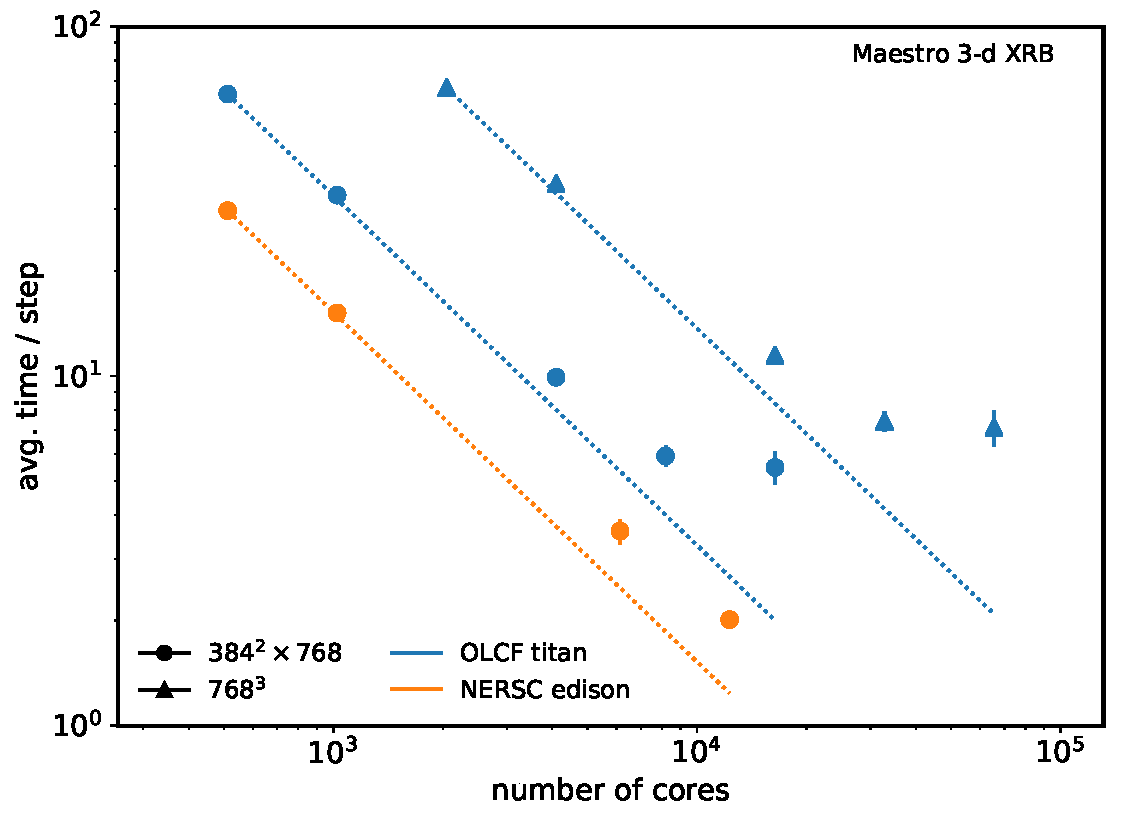
\includegraphics[width=0.48\linewidth]{titan_edison_maestro_scaling}
\begin{minipage}[b]{0.48\linewidth}
\caption{\label{fig:maestro_scaling} \maestro\ strong scaling on NERSC
  edison and OLCF titan for a 3-d XRB problem.  Two different problem
  sizes are shown.\vspace{2em}}
\end{minipage}
\end{figure}

\begin{figure}[t]
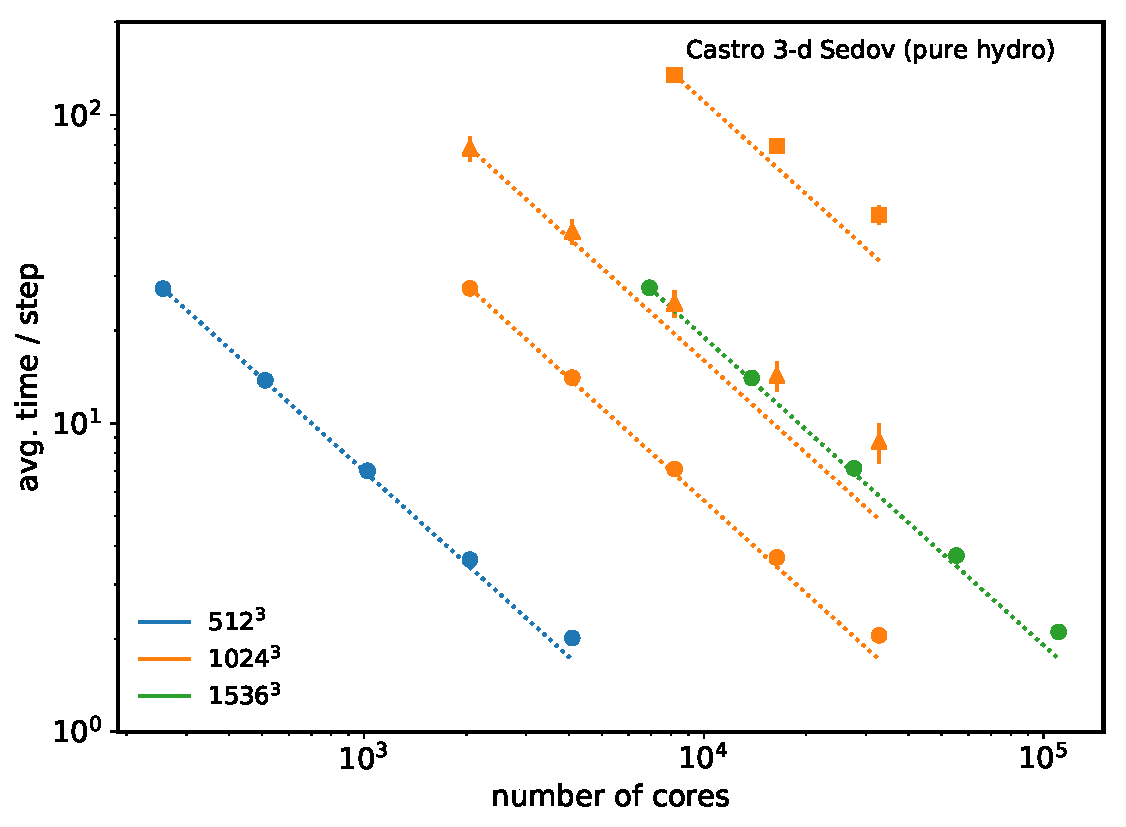
\includegraphics[width=0.48\linewidth]{sedov_scaling}
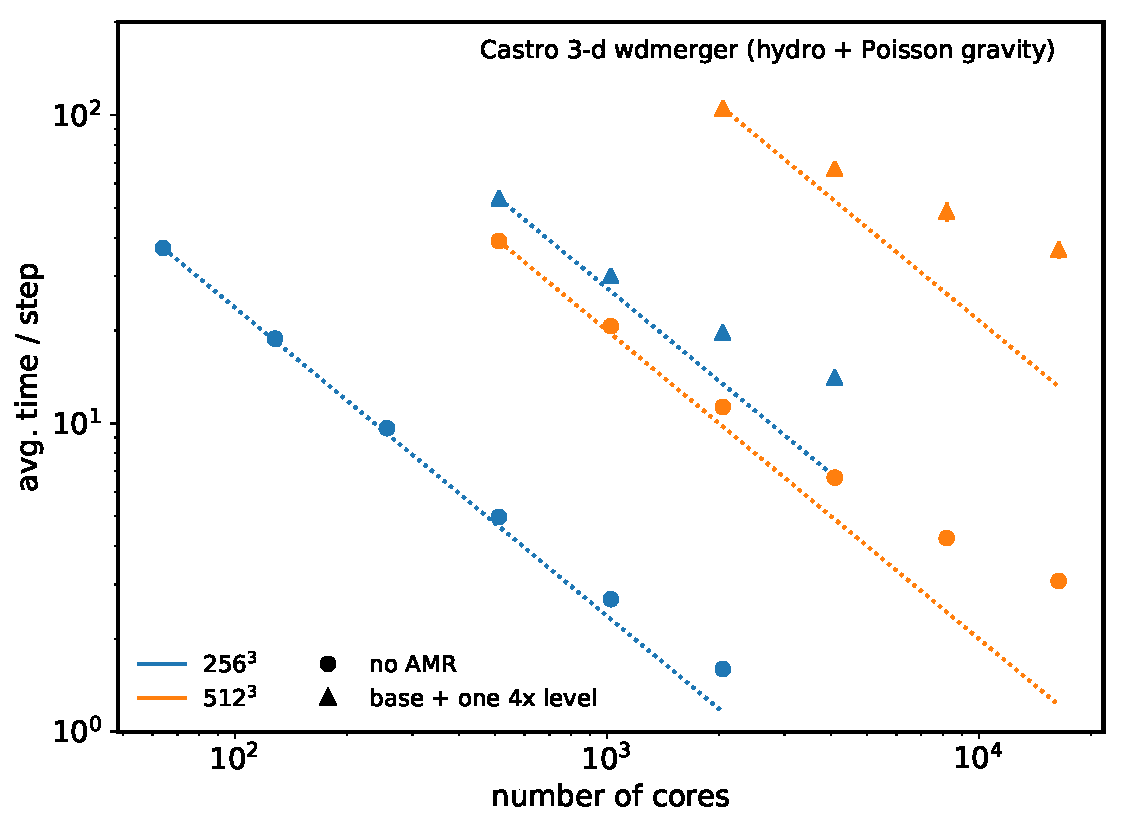
\includegraphics[width=0.48\linewidth]{wdmerger_scaling} \\
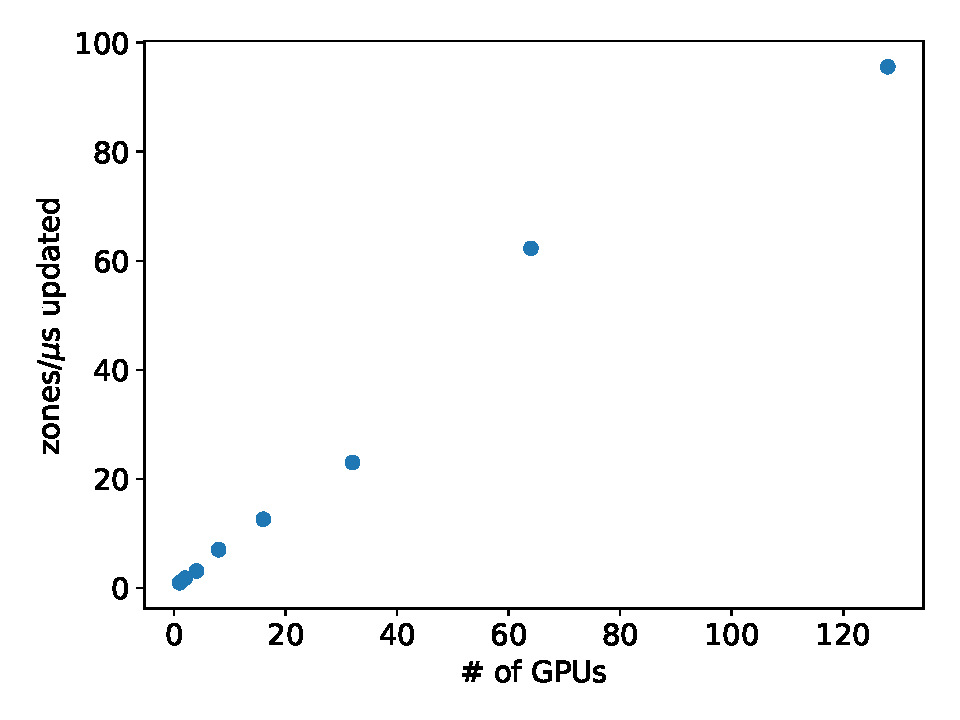
\includegraphics[width=0.48\linewidth]{summitdev_scaling}
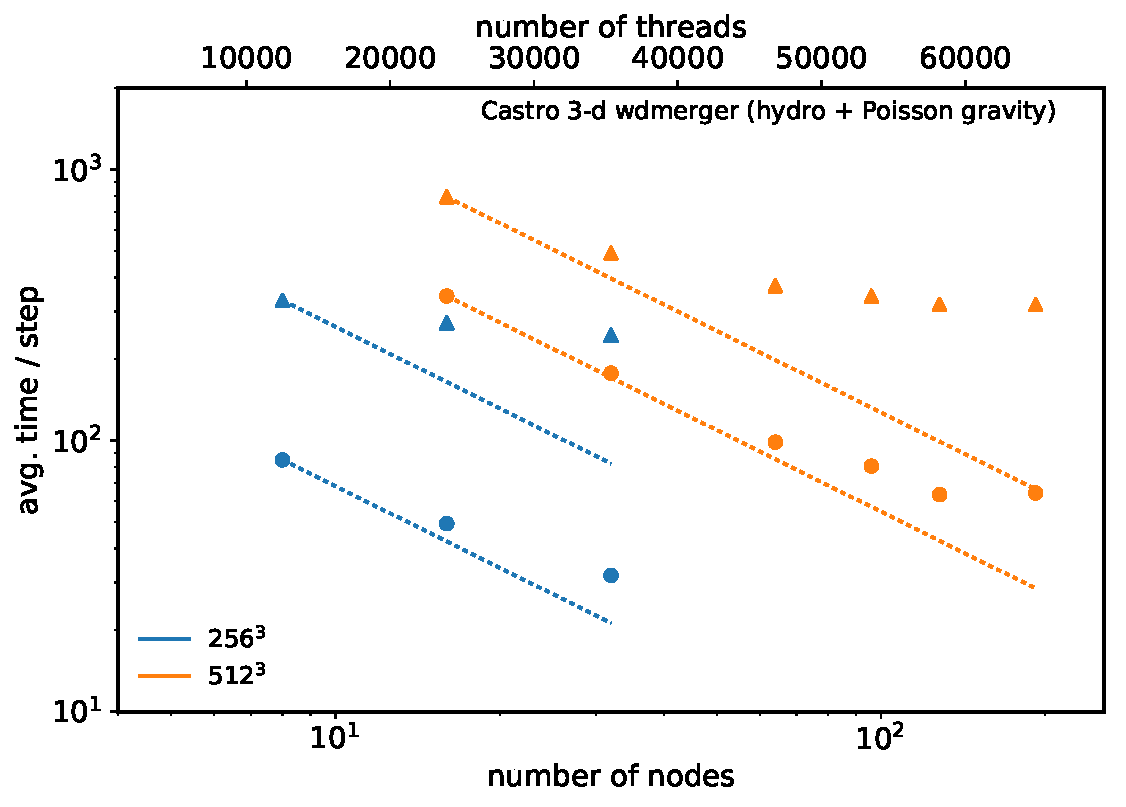
\includegraphics[width=0.48\linewidth]{cori_scaling}
\caption{\label{fig:scaling} (left) \maestro\ strong scaling on NERSC edison
and OCLF titan for a 3-d XRB problem.  Two different problem sizes are show.
(right) \starlord\ scaling across nodes on the OLCF summitdev platform, using
up to 4 GPUs per node.}
\end{figure}

Figure~\ref{fig:scaling} shows strong scaling for \maestro\ on the 3-d
XRB problem.  We see that the code scales well to $\mathcal{O}(10^4)$
processors.  The main limitation to the scaling at the moment are the
multigrid solves used to enforce the projection (in particular the
nodal solver).  \maestro\ also does not yet take advantage of the
tiling capabilities offered in \amrex.  These will be addressed in the
future as we port \maestro\ to the C++ \amrex\ codebase to take advantage
of ongoing development.

Castro scaling is a placeholder...

Our latest focus has been on GPU ports of our application codes.  A
small proxy app, \starlord, was created from \castro\ with just the
hydrodynamics and stellar equation of state.  It uses a simple
method-of-lines formulation of the hydrodynamics and advects 13
nuclear species in addition to the hydrodynamics.  To offload work on
GPUs, GPU support was added directly into \amrex.  In \amrex, grids
consist of a number of boxes that enable domain decomposition for
parallelism.  An iterator loops over all of the boxes at the same
level of refinement and passes a data pointer into a Fortran kernel
function where the work is done. For the simulation state data that
resides in each box, we have modified the memory allocator so that it
can use a CUDA allocator (either device or managed memory).  The
domain iterator is configured to handle data motion to and from the
device, so that the compute kernels can operate on data which is
presumed to already be there, and the computation is decoupled from
the memory management. Computation on the data can then be performed
with OpenACC, CUDA Fortran, or (more recently) OpenMP 4.5. We have
also built CUDA compute support into \amrex\ so that a compute kernel
can be transparently operated on using CUDA Fortran without
substantially modifying the kernels (and we anticipate using a similar
strategy to use OpenACC and/or OpenMP in the future). This helps
ensure that we can continue to maintain performance portability in our
simulation codes, by decoupling the physics algorithms from the
backend support used to implement them on various compute
architectures.\MarginPar{add CPU time for reference}

Figure~\ref{fig:scaling} shows the performance of \starlord\ on the
summitdev platform at OLCF\footnote{summitdev consists of 2 IBM Power8
  processors and 4 Nvidia Pascal GPUs per node.}.  The highest GPU
count (128) corresponds to 32 nodes on summitdev.  We see a nearly
linear speedup with the number of GPUs, indicating good weak scaling
on this machine.  Efforts are underway to complete the port of the GPU
developments into \castro.

\begin{figure}[t]
\centering
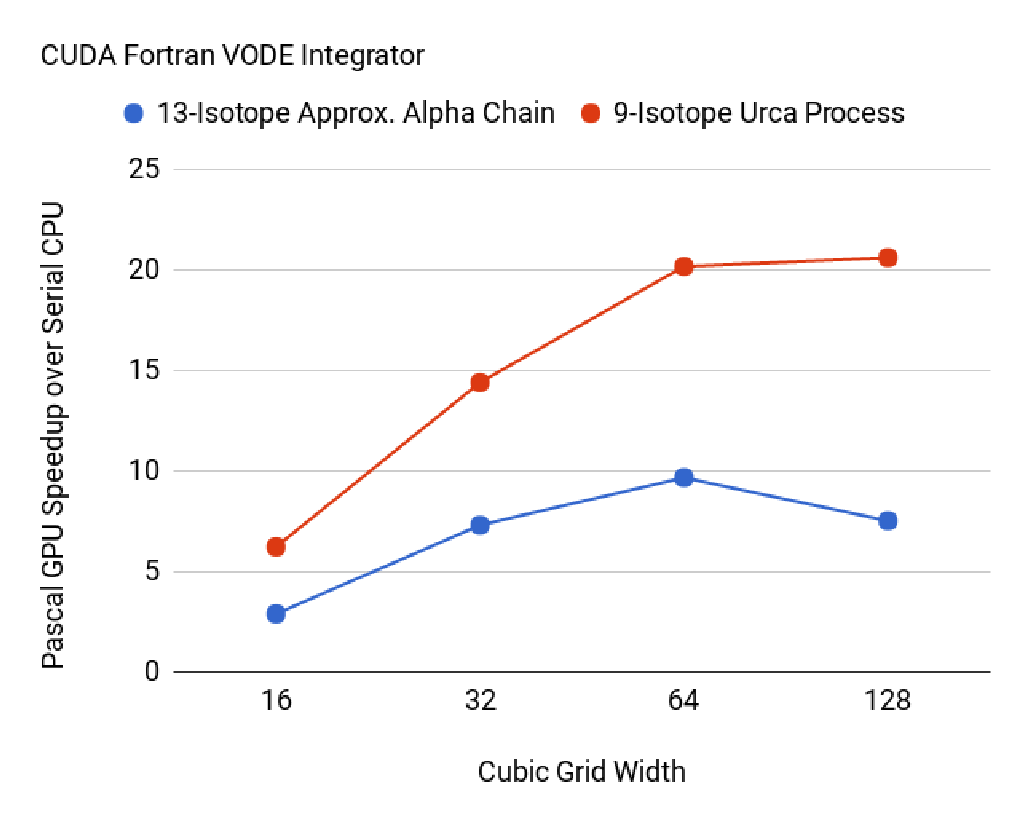
\includegraphics[width=0.48\linewidth]{CUDA-Fortran-VODE-Integrator}
\begin{minipage}[b]{0.48\linewidth}
\caption{\label{fig:cudaode} GPU speed up over single CPU core for two
  reaction networks.  The 13-isotope alpha-chain is a
  potential network for the sub-Chandra simulations we propose here.
  The 9-isotope Urca network is used for our Urca simulations.  A
  variety of grid sizes were used, $16^3$, $32^3$, $64^3$, and
  $128^3$.  In all cases, we see significant speed up on the GPU
  vs.\ a single core.  These speed-up numbers are from our testbed
  workstation with a Titan X Pascal board and Intel Xeon X5650 processors.}
\end{minipage}
\end{figure}

A parallel effort is porting our microphysics, in particular reaction
networks to GPUs.  Our strategy is to do the entire ODE integration on
the GPU, i.e., the data for a patch of zones is passed to the GPU, all
righthand size and Jacobian evaluations and the timestepping itself is
done on the GPU and once all zones are burned, we access the data as
needed on the CPU.  To enable this, we ported our workhorse ODE
integrator (VODE~\cite{vode}) to CUDA Fortran. This required extensive
rewrites of the internals of VODE, which was originally written using
Fortran 77 syntax unsupported by CUDA Fortran. Accelerating VODE with
CUDA Fortran has proven successful, and we now see significant
performance gains with the CUDA version of our reaction networks, even
for moderate sized networks (a 13-isotope standard network).
Figure~\ref{fig:cudaode} shows the speed-ups on a GPU vs.\ single CPU
core.



\section{Some science results}

\begin{figure}[t]
\centering 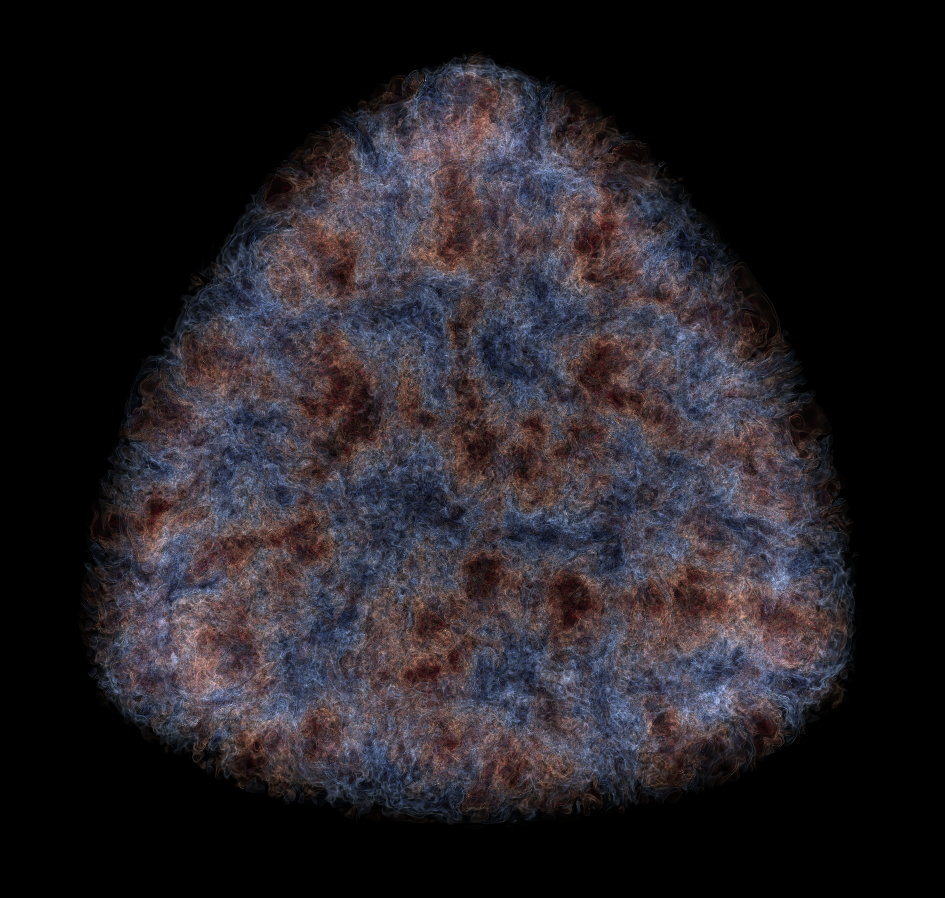
\includegraphics[height=1.8in]{subch_h}
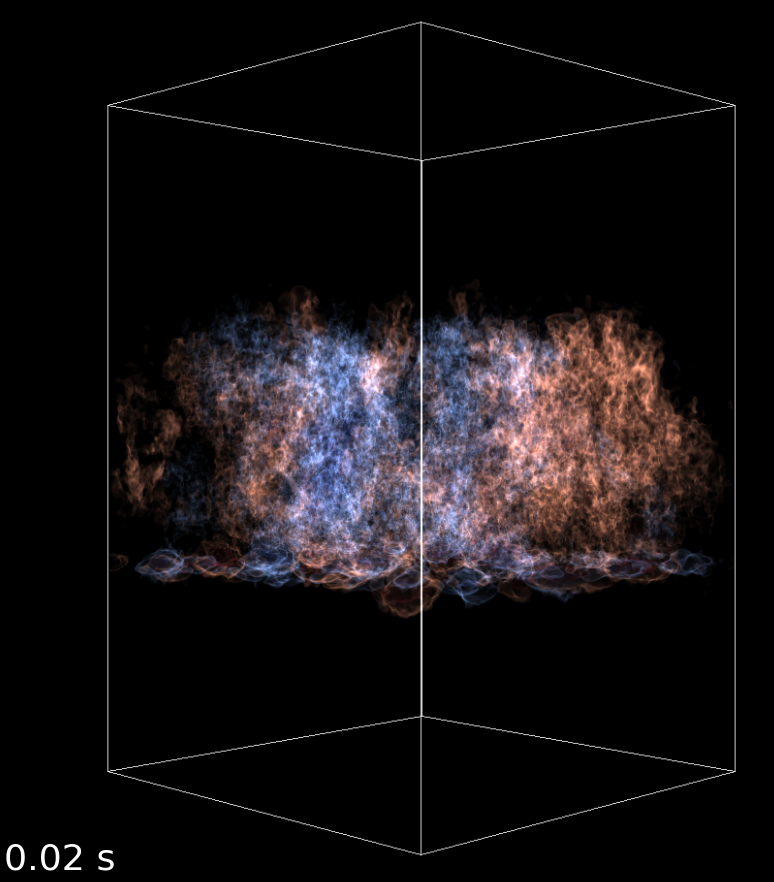
\includegraphics[height=1.8in]{xrb_compact}
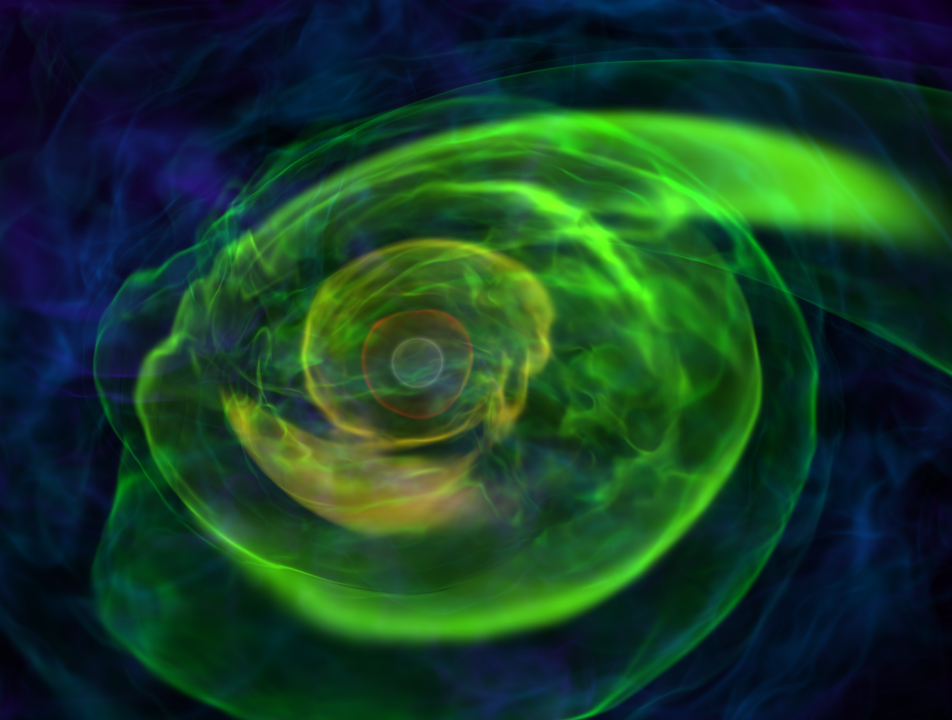
\includegraphics[height=1.8in]{wdmerger_08030_new}
\caption{\label{fig:current-runs} (left) Convective plumes in a
  \maestro\ sub-Ch calculation. (center) Vertical velocity showing the
  convective structure in a \maestro\ XRB calculation. (right)
  Snapshot of a \castro\ simulation of the merger of two white dwarfs,
  with 0.90 and 0.81 solar masses. The contours represent density
  levels.}
\end{figure}

Figure~\ref{fig:current-runs} shows some of our recent science
simulations.  The left panel is an image of convection in the helium
layer on a sub-Chandra white dwarf.  This is part of a study of the
early stages of the double detonation SNe Ia model.  Using \maestro,
we are able to model the convection in the He layer for many turnover
times and saw a range of outcomes depending on the mass of the white
dwarf and He layer, including a global He-nova-like behavior where the
entire layer runsway together and localized
burning~\cite{subchandra2}.

The middle figure shows convection in a H/He layer on a neutron star,
as a model of the early burning in an XRB.  This \maestro\ model was
the first 3D model of convection for this problem~\cite{xrb3}.  This
study showed that the convective field became fully turbulent,
achieving a Kolmogorov spectrum, and the overall dynamics was very
different than our earlier 2-d simulations.

The rightmost image is the coalesced remains of the merger of a
0.9~$M_\odot$ and 0.6~$M_\odot$ WD performed with \castro.  This used
the developments from \cite{wdmergerI}.  Our primary focus with this
suite of simulations is understanding the numerical sensitivity of
mergers and collisions on the burning that takes place.


\section{Summary and future development}

We described our suite of astrophysics codes built on the
\amrex\ framework.  These codes were developed to model problems in
stellar astrophysics spanning from low speed convection to explosive
burning.  A major theme of the codes is the open development model,
with the code development done on github and all problem files needed
to recreate any science results freely available.  Future development
efforts for \maestro\ include higher-order hydrodynamics and
time-integration and rotation.  For \castro, we are investigating
strong coupling between hydrodynamics and reactions, new solvers
(including MHD), and finishing the GPU port.



\ack The work at Stony Brook was supported by DOE/Office of Nuclear
Physics grant DE-FG02-87ER40317 and NSF award AST-1211563.  An award
of computer time was provided by the Innovative and Novel
Computational Impact on Theory and Experiment (INCITE) program.  This
research used resources of the Oak Ridge Leadership Computing Facility
at the Oak Ridge National Laboratory, which is supported by the Office
of Science of the U.S. Department of Energy under Contract
No.\ DE-AC05-00OR22725.  We appreciate the efforts of the OLCF (and in
particular Fernanda Foertter) in organizing the GPU hackathons.  This
research used resources of the National Energy Research Scientific
Computing Center, which is supported by the Office of Science of the
U.S. Department of Energy under Contract No.\ DE-AC02-05CH11231.
Results in this paper were obtained using the high-performance LIred
computing system at the Institute for Advanced Computational Science
at Stony Brook University, which was obtained through the Empire State
Development grant NYS \#28451.  The GPU work benefited from a grant of
an Titan X Pascal board from Nvidia Corp through the GPU Grant
Program.  This research has made use of NASA's Astrophysics Data
System Bibliographic Services.

\section*{References}

\bibliographystyle{iopart-num}
\bibliography{ws}


\end{document}
